\documentclass{beamer}

\usepackage{tikz}
\usepackage{listings}
\usetikzlibrary{arrows.meta}
\usetikzlibrary{calc,positioning,arrows}

%Import the style of the document
\usetheme{Madrid}
\usecolortheme{default}

\setbeamercolor{frametitle}{bg=gray!0!black, fg=white}

\setbeamercolor{title}{fg=white, bg=gray!0!black}
\setbeamertemplate{footline}{}
\setbeamertemplate{navigation symbols}{}
\setbeamertemplate{footline}{
  \hfill
  \usebeamercolor[fg]{page number in head/foot}
  \usebeamerfont{page number in head/foot}
  \insertframenumber\hspace{0.3cm}
  \vspace{0.2cm}
}

\setbeamercolor{item}{fg=black}
\setbeamercolor{itemize item}{fg=black}
\setbeamercolor{itemize subitem}{fg=black}


\title{Programming Scalable Systems}
\author{
Rubén García-Patos Benito (helarteDeProgrmar)\\[0.5em] Germán Ruiz Cabello (geermanruuiz)\\[0.5em] Alejandro Soriano Compta (Alexsq1)}
\date{May, 2025}

\begin{document}
\lstdefinelanguage{elixir}{
    morekeywords={
      after,
      alias,
      and,
      case,
      catch,
      cond,
      def,
      defimpl,
      defmacro,
      defmacrop,
      defmodule,
      defoverridable,
      defp,
      defprotocol,
      defstruct,
      do,
      else,
      end,
      false,
      fn,
      for,
      if,
      import,
      in,
      nil,
      not,
      or,
      quote,
      raise,
      receive,
      require,
      rescue,
      true,
      try,
      unless,
      use,
      when,
      with,
      unquote,
      defdelegate
    },
    emph={iex},
    alsoletter={:},
    sensitive=true,
    morecomment=[l]{\#},
    morecomment=[n]{/*}{*/},
    morecomment=[n]{@doc\ "}{"},
    morecomment=[n]{@doc\ """}{"""},
    string=[b]",
    morestring=[b]'
}

\begin{frame}[plain]
  \titlepage
\end{frame}

\begin{frame}{Design}

\begin{figure}[H]
\begin{center}
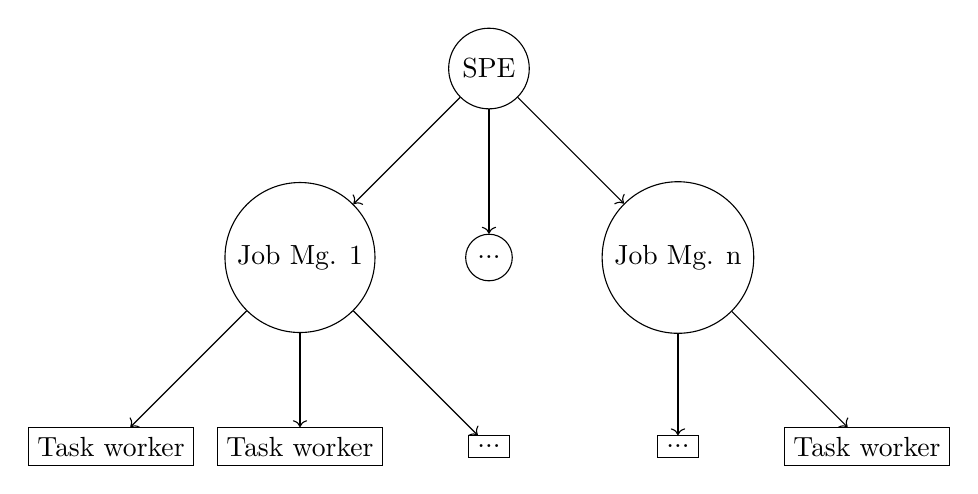
\begin{tikzpicture}[node distance=2.4cm, auto]
  \node[draw, circle] (SPE) {SPE};
  \node[draw, circle, below of=SPE] (JM2) {...};
  \node[draw, circle, left of=JM2] (JM1) {Job Mg. 1};
  \node[draw, circle, right of=JM2] (JM3) {Job Mg. n};
  
  \node[draw, rectangle, below of=JM1] (TW11) {Task worker};
  \node[draw, rectangle, right of=TW11] (TW12) {...};
  \node[draw, rectangle, right of=TW12] (TW13) {...};
  \node[draw, rectangle, left of=TW11] (TW14) {Task worker};

  \node[draw, rectangle, right of=TW13] (TWn) {Task worker};
  
  \draw[->] (SPE) to (JM1) ;
  \draw[->] (SPE) to (JM2) ;
  \draw[->] (SPE) to (JM3) ;

  \draw[->] (JM1) to (TW11) ;
  \draw[->] (JM1) to (TW12) ;
  \draw[->] (JM3) to (TW13) ;
  \draw[->] (JM1) to (TW14) ;

  \draw[->] (JM3) to (TWn) ;

\end{tikzpicture}
\end{center}
\end{figure}
\end{frame}

\begin{frame}{Messages SPE}
    \begin{table}[]
        \centering
        \begin{tabular}{|c|c|c|}
        \hline
        From & To & Message \\
        \hline
        \hline
        \hline
        Client & \textbf{SPE} & start \\
        Client & \textbf{SPE} & submit\_job \\
        Client & \textbf{SPE} &  start\_job \\
        \textbf{SPE} & Job manager & start \\
        \textbf{SPE} & Job manager &  start\_one\_task \\
        \hline
        \end{tabular}
    \end{table}
\end{frame}

\begin{frame}{Messages Job Manager}

    \begin{table}[]
        \centering
        \begin{tabular}{|c|c|c|}
        \hline
        From & To & Message \\
        \hline
        \hline
        \hline
        \textbf{Job Manager} & SPE & existing\_worker \\
        \textbf{Job Manager} & SPE & one\_task\_finished \\
        \textbf{Job Manager} & SPE & job\_finished \\
        \textbf{Job Manager} & Task worker & start \\
        
        \hline
        \end{tabular}
    \end{table}

\end{frame}

\begin{frame}{Task worker}

    \begin{table}[]
        \centering
        \begin{tabular}{|c|c|c|}
        \hline
        From & To & Message \\
        \hline
        \hline
        \hline
        \textbf{Task worker} & Job Manager & task\_finished \\
        \hline
        \end{tabular}
    \end{table}
\end{frame}

\begin{frame}{Summary of messages}

\begin{figure}[H]
\begin{center}
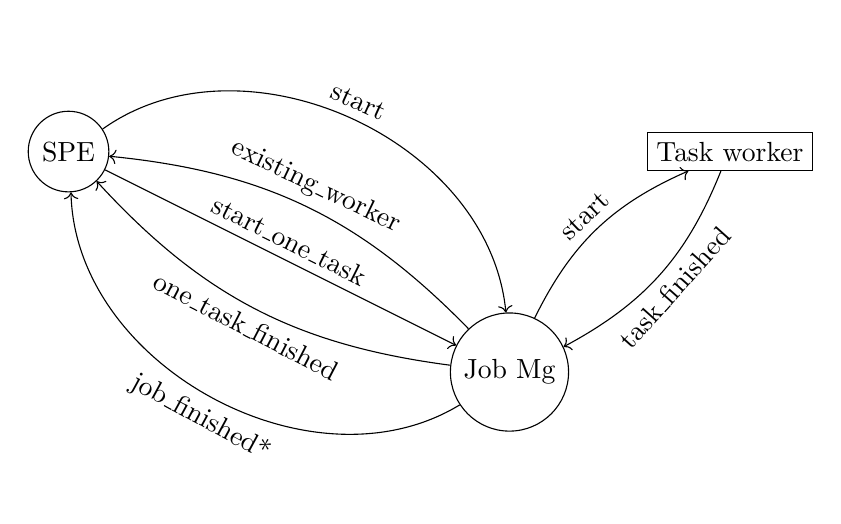
\begin{tikzpicture}[node distance=2.8cm, auto]
  
  \node[draw, circle] (SPE) {SPE};
  \node[circle, right of=SPE] (aux1) {};
  \node[circle, right of=aux1] (aux2) {};
  \node[draw, circle, below of=aux2] (JM) {Job Mg};
  
  \node[circle, right of=JM] (aux3) {};
  \node[draw, rectangle, above of=aux3] (TW) {Task worker};

  \draw[->] (SPE) to[bend left=60] node[midway, sloped, above] {start} (JM);
  \pause
  \draw[->] (JM) to[bend right=20] node[midway, sloped, above] {existing\_worker} (SPE);
  \pause
  \draw[->] (SPE) to[bend left=0] node[midway, sloped, above] {start\_one\_task} (JM);
  \pause
  \draw[->] (JM) to[bend left=20] node[midway, sloped, above] {start} (TW);
  \pause
  \draw[->] (TW) to[bend left=20] node[midway, sloped, below] {task\_finished} (JM);
  \pause
  \draw[->] (JM) to[bend left=20] node[midway, sloped, below] {one\_task\_finished} (SPE);
  \pause
  \draw[->] (JM) to[bend left=60] node[midway, sloped, below] {job\_finished*} (SPE);
\end{tikzpicture}
\end{center}
\end{figure}
\end{frame}

\begin{frame}{Implementation details}

    \begin{table}[]
        \centering
        \begin{tabular}{|c|c|}
        \hline
        Element & Implementation \\
        \hline
        \hline
        \hline
        \textbf{SPE} & GenServer \\
        \textbf{Job manager} & GenServer \\
        \textbf{Task worker} & Task \\
        \hline
        \end{tabular}
    \end{table}
    
\end{frame}

\begin{frame}{State SPE}

\begin{itemize}
    \item num\_workers (int)
    \item current\_workers (int)
    \item pid\_queued\_jobs (list of PIDs)
    \item jobs (map)
    \item next\_unique\_id (int)
\end{itemize}
    
\end{frame}

\begin{frame}{State Job Manager}
    \begin{itemize}
        \item job\_id (int)
        \item name (string)
        \item server\_pid (PID)
        \item queued (list of tasks)
        \item blocked (list of tasks)
        \item running (map of tasks)
        \item status (atom)
        \item results (map of task-results)
    \end{itemize}
\end{frame}

\begin{frame}[fragile]{Task implementation}

\begin{lstlisting}[language=elixir]
    Task.start(
        fn -> 
            run(name, fun, input, timeout, caller) 
        end
    )

    defp execute_with_timeout(function, input, ms) 
    defp execute_without_timeout(function, input) 
    defp safe_execution(function, input)
\end{lstlisting}
   
\end{frame}
\end{document}